A otimização híbrida surge como uma abordagem eficaz para lidar com problemas de otimização global caracterizados por funções objetivo de elevado custo computacional. Nesses cenários, a aplicação direta de métodos clássicos de otimização torna-se impraticável, motivando o desenvolvimento de estratégias que reduzam o número de avaliações reais da função \cite{Jones1998,Forrester2008}.

O princípio fundamental da otimização híbrida consiste na combinação de modelos aproximados (\textit{surrogates}) com estratégias de busca global. Em particular, a maior parte das avaliações diretas da função objetivo é substituída por predições fornecidas por um modelo de baixo custo computacional, enquanto avaliações reais são realizadas de forma seletiva e orientada. Essa estratégia permite reduzir significativamente o custo computacional total do processo de otimização, sem comprometer a capacidade de exploração global do espaço de busca \cite{Jones1998}.

Neste trabalho, adota-se uma estratégia híbrida de otimização baseada em aprendizado de máquina, fundamentada no método \textit{Efficient Global Optimization} (EGO). Esta abordagem será combinada com um algoritmo genético para assegurar a convergência a um ótimo global da função mono-objetivo.

\subsection{Problema mono-objetivo}

Um problema de otimização mono-objetivo ($SOO - Single \; Objective \;Optimization$) busca um resultado ótimo em um ponto do espaço de projeto que minimiza (ou maximiza) apenas uma função objetivo \cite{moreira}. Semelhante aos problemas multiobjetivos, a formulação de um problema mono-objetivo inclui um conjunto de restrições. Essas restrições representam condições que qualquer solução considerada viável deve obrigatoriamente satisfazer. Desse modo, a busca pela solução ótima ocorre apenas dentro do espaço de soluções que atendam às restrições estabelecidas. O conjunto de equações representado em \eqref{eq:problema_otimizacao} apresenta a forma genérica de um problema mono-objetivo:

\begin{equation}
\left\{\; \;
\begin{aligned}
& \min f(\textbf{X}), \\[0.3em]
& g_i(\textbf{X}) \le 0, \quad i = 1, 2, \dots, J, \\[0.3em]
& h_j(\textbf{X}) = 0, \quad j = 1, 2, \dots, K, \\[0.3em]
& x_i^L \le x_i \le x_i^U, \quad i = 1, 2, \dots, n.
\end{aligned}
\right.
\label{eq:problema_otimizacao}
\end{equation}
\vspace{1em}

A formulação envolve uma função objetivo $f(\textbf{X})$, onde X representa o vetor das variáveis de projeto. As inequações $g_j (\textbf{X})$, as equações $h_k (\textbf{X})$ e os limites laterais $x_i^L$ e $x_i^U$ correspondem às restrições que delimitam o espaço de busca viável. Os índices $j$, $k$ e $i$ identificam, respectivamente, as restrições de desigualdade, de igualdade e o intervalo de busca, enquanto $J$, $K$ e $n$ representam as quantidades totais desses elementos.

\subsection{Efficient Global Optimization (EGO)}
 
 Proposto por Jones, Schonlau e Welch \cite{Jones1998}, o EGO é um método de otimização global voltado para problemas em que a avaliação da função objetivo tem alto custo computacional. A ideia central do EGO é reduzir o número de avaliações diretas da função \textit{black-box} por meio de um modelo substituto (do inglês \textit{surrogate}), que aprende uma aproximação da função a partir de um conjunto inicial de amostras e é atualizado iterativamente ao longo do processo.

Em cada iteração, o EGO ajusta um modelo probabilístico (tipicamente um Processo Gaussiano/\textit{kriging}) e utiliza uma função de aquisição para decidir qual ponto deve ser avaliado a seguir. Essa função de aquisição quantifica um critério de utilidade que balanceia dois objetivos concorrentes: (i) explorar regiões do espaço de busca, onde a incerteza do modelo é alta (exploração) e (ii) intensificar a busca em regiões promissoras, onde a predição indica valores baixos da função objetivo (intensificação). Uma escolha clássica de função de aquisição no EGO é o \textit{Expected Improvement} (EI), que mede a melhoria esperada em relação ao melhor valor observado até o momento \cite{Jones1998,Shahriari2016}.

Na perspectiva de aprendizado de máquina, o EGO pode ser interpretado como uma arquitetura de aprendizado ativo. Diferentemente de abordagens passivas, nas quais o modelo é treinado sobre um conjunto fixo de dados, o EGO seleciona iterativamente novos pontos de amostragem com base em um critério de decisão que maximiza a expectativa de melhoria ou o ganho informacional. Essa interpretação se alinha à literatura de otimização Bayesiana e projeto sequencial de experimentos, na qual funções de aquisição são tratadas como utilidades para decidir novas avaliações com orçamento limitado \cite{Shahriari2016,SCHULZ20181, Snoek2012}.

Esse tipo de abordagem também aparece em aplicações recentes de projeto computacional: Deng Paulson e Messner (\cite{Deng2026_MetamaterialAL}) propõem um método \textit{gradient-free} para o projeto de metamateriais que usa a Regressão por Processo Gaussiano (GPR) para representar o campo de densidade, comprime a representação (matriz de covariância) para reduzir a dimensionalidade e, no espaço comprimido, emprega um método de \textit{active learning} (BADS — \textit{Bayesian Adaptive Direct Search}) para explorar o espaço de projeto de forma eficiente \cite{Deng2026_MetamaterialAL}.

\subsection{Regressão por Processo Gaussiano (GPR)}


No contexto do EGO, o modelo substituto é tipicamente formulado por meio de Regressão por Processo Gaussiano (GPR), também associada à tradição de \textit{kriging} na literatura de experimentos computacionais e superfícies de resposta \cite{Jones1998,Shahriari2016}. Diferentemente de modelos paramétricos, que assumem previamente uma forma funcional fixa, o GPR adota uma perspectiva Bayesiana não paramétrica, na qual se define uma distribuição de probabilidade sobre funções. Essa característica é particularmente adequada em problemas de otimização nos quais a função objetivo é desconhecida, cara de avaliar e pode apresentar comportamento não linear ou multimodal \cite{NIPS1995_7cce53cf,SCHULZ20181,Shahriari2016}.

Formalmente, assume-se que a função latente \(f(\mathbf{x})\) segue um processo gaussiano,
\begin{equation}
    f(\mathbf{x}) \sim \mathcal{GP}\!\big(m(\mathbf{x}),\,k(\mathbf{x},\mathbf{x}')\big),
\end{equation}
em que \(m(\mathbf{x})\) é a função média e \(k(\mathbf{x},\mathbf{x}')\) é a função de covariância, ou \textit{kernel}. No GPR, o \textit{kernel} desempenha papel central, pois é ele que define a estrutura de dependência entre os pontos do espaço de entrada. Em termos de modelagem, deseja-se especificar covariâncias de modo que pontos com entradas próximas produzam predições semelhantes \cite{NIPS1995_7cce53cf}. Assim, o \textit{kernel} codifica hipóteses iniciais sobre regularidade, suavidade e escala de variação da função, além de controlar como a informação observada em um ponto se propaga para regiões vizinhas do domínio \cite{NIPS1995_7cce53cf,SCHULZ20181}. Em problemas práticos, as observações podem ser descritas por
\begin{equation}
    y = f(\mathbf{x}) + \varepsilon,
\end{equation}
onde \(\varepsilon\) representa ruído observacional, usualmente modelado como gaussiano \cite{SCHULZ20181,Shahriari2016}.

Dado um conjunto de dados \(D=\{X,\mathbf{y}\}\), o GPR fornece, para qualquer ponto não observado \(\mathbf{x}\), uma distribuição preditiva gaussiana caracterizada por média \(\mu(\mathbf{x})\) e variância \(\sigma^2(\mathbf{x})\). Na forma clássica, a predição posterior pode ser escrita como
\begin{equation}
    \mu(\mathbf{x}) = K(\mathbf{x},X)\big(K(X,X)+\sigma_\varepsilon^2 I\big)^{-1}\mathbf{y},
\end{equation}
\begin{equation}
    \sigma^2(\mathbf{x}) = k(\mathbf{x},\mathbf{x}) - K(\mathbf{x},X)\big(K(X,X)+\sigma_\varepsilon^2 I\big)^{-1}K(X,\mathbf{x}),
\end{equation}
em que \(K(X,X)\) é a matriz de covariância entre os pontos amostrados \cite{NIPS1995_7cce53cf}. A média preditiva expressa a melhor estimativa do valor da função, enquanto a variância quantifica a incerteza associada ao modelo em cada região do domínio. Como ambas dependem diretamente da função de covariância, a escolha do \textit{kernel} afeta simultaneamente a qualidade da aproximação e a forma como a incerteza é distribuída no espaço de busca \cite{NIPS1995_7cce53cf}.

Essa quantificação explícita de incerteza é precisamente o que torna o GPR particularmente apropriado para o EGO. Como a otimização Bayesiana é um procedimento sequencial baseado em modelo probabilístico, o \textit{surrogate} precisa não apenas aproximar a função objetivo, mas também indicar onde essa aproximação é menos confiável \cite{Shahriari2016}. Nesse sentido, \(\mu(\mathbf{x})\) sustenta a intensificação em regiões promissoras, ao passo que \(\sigma(\mathbf{x})\) viabiliza a exploração de regiões ainda pouco conhecidas. No EGO, essa dualidade é explorada por funções de aquisição como o \textit{Expected Improvement}, que utilizam simultaneamente predição e incerteza para decidir a próxima avaliação cara da função \cite{Jones1998,Shahriari2016}.

Além disso, o desempenho do GPR depende da escolha do \textit{kernel} e de seus hiperparâmetros. Em Williams e Rasmussen, por exemplo, os parâmetros da covariância controlam a escala das correlações locais, a contribuição de componentes lineares e de viés, bem como a variância do ruído; em particular, diferentes pesos por dimensão permitem refletir a relevância relativa de cada variável de entrada \cite{NIPS1995_7cce53cf}. Assim, no EGO, o GPR atua como um \textit{surrogate} probabilístico capaz de combinar flexibilidade funcional, interpolação não linear e quantificação de incerteza, reduzindo o número de avaliações reais necessárias em problemas de otimização de alto custo computacional \cite{Jones1998,Shahriari2016}.
\subsection{Critério de aquisição: \textit{Expected Improvement} (EI)}

Considere um conjunto de amostras $X=\{\mathbf{x}_1,\ldots,\mathbf{x}_n\}$ e respostas $Y=\{y_1,\ldots,y_n\}$, obtidas ao avaliar a função cara $F(\cdot)$ a ser minimizada. Denote o melhor valor observado por:

\begin{equation}
f_{\min}=\min\{y_1,y_2,\ldots,y_n\}.
\end{equation}

Assumindo que o \textit{surrogate} fornece, para cada $\mathbf{x}$, uma distribuição preditiva normal

\begin{equation}
Y(\mathbf{x}) \sim \mathcal{N}\big(\mu(\mathbf{x}),\,\sigma^2(\mathbf{x})\big),
\end{equation}

em que $Y(\mathbf{x})$ é a variável aleatória que modela o valor da função objetivo real. $\mathcal{N}$ Indica que a distribuição é normal (gaussiana), $\mu(\mathbf{x})$ representa a melhor estimativa do modelo para o valor da função objetivo. $\sigma^2(\mathbf{x})$ é a variância da distribuição preditiva. Sua raiz quadrada, 
$\sigma(\mathbf{x})$, é o desvio padrão, que quantifica a incerteza do modelo. Em seguida define-se a melhoria aleatória

\begin{equation}
I(\mathbf{x})=\max\big(f_{\min}-Y(\mathbf{x}),\,0\big),
\end{equation}

e a função de aquisição como sua esperança:

\begin{equation}
\mathrm{EI}(\mathbf{x})=\mathbb{E}[I(\mathbf{x})].
\end{equation}

No caso gaussiano, obtém-se uma forma fechada \cite{Jones1998} para a função de aquisição:

\begin{equation}
\mathrm{EI}(\mathbf{x})=
\big(f_{\min}-\mu(\mathbf{x})\big)\,
\Phi\!\left(\frac{f_{\min}-\mu(\mathbf{x})}{\sigma(\mathbf{x})}\right)
+\sigma(\mathbf{x})\,
\phi\!\left(\frac{f_{\min}-\mu(\mathbf{x})}{\sigma(\mathbf{x})}\right),
\label{eq:ei_closed_form}
\end{equation}

onde $\Phi(\cdot)$ e $\phi(\cdot)$ são, respectivamente, a CDF (\textit{Cumulative Distribution Function}) e a PDF (\textit{Probability Density Function}) da normal padrão. A Equação~\eqref{eq:ei_closed_form} é o ponto-chave: o termo com $\Phi(\cdot)$ favorece intensificação quando a média predita melhora $f_{\min}$, enquanto o termo com $\phi(\cdot)$ cresce com $\sigma(\mathbf{x})$, favorecendo exploração em regiões incertas \cite{Jones1998,Shahriari2016}.

\subsection{Otimizador interno}\label{sec:otm_interno}

Uma vez construído o modelo substituto (\textit{surrogate} model), a maximização do \textit{Expected Improvement} (EI) que é expresso pela Equação~\eqref{eq:ei_closed_form} é conduzida por um otimizador interno baseado em metaheurística. Neste trabalho, adotou-se um Algoritmo Genético (AG), implementado por meio da biblioteca \textsc{MEALPY} \cite{van2023mealpy, van2023groundwater}, cujos fundamentos e parametrização são descritos a seguir.

O Algoritmo Genético é uma metaheurística inspirada nos mecanismos da evolução natural e na seleção darwiniana \cite{holland1992}. Seu funcionamento básico consiste em evoluir iterativamente uma população de soluções candidatas (indivíduos) por meio dos operadores de \textbf{seleção}, \textbf{cruzamento} e \textbf{mutação}, preservando as características mais promissoras ao longo das gerações. Um fluxograma esquemático do processo é apresentado na Figura~\ref{fig:fluxograma_AG}.

\begin{figure}[H]
  \centering
  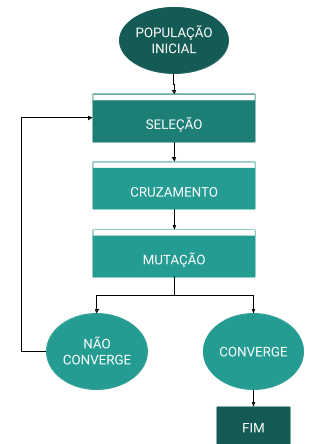
\includegraphics[width=0.4\textwidth]{figuras/fluxograma_AG.png}
  \caption{Fluxograma representativo do Algoritmo Genético.}
  \label{fig:fluxograma_AG}
\end{figure}

O AG inicia com uma população aleatória de indivíduos, cada um representando um ponto no espaço de busca. A cada geração, os indivíduos são avaliados segundo uma função de aptidão. Os mais aptos têm maior probabilidade de serem selecionados para reprodução, gerando novos indivíduos que gradualmente convergem para regiões de maior interesse.

\subsubsection{Operadores genéticos adotados}

\textbf{Seleção por roleta}: Utilizou-se o método da roleta (\textit{roulette wheel selection}), no qual cada indivíduo recebe uma probabilidade de seleção proporcional à sua aptidão relativa. Isso permite que indivíduos menos aptos ainda possam ser escolhidos, mantendo a diversidade populacional e reduzindo o risco de convergência prematura \cite{linden}.

\textbf{Cruzamento linear}: Dois indivíduos selecionados \( p_0 \) e \( p_1 \) são combinados para gerar três descendentes por combinação linear de suas variáveis de projeto:

\begin{equation}
\begin{aligned}
{des}_{a,k} &= 0{,}50 \cdot p_{0,k}^{t} + 0{,}50 \cdot p_{1,k}^{t},\\[2pt]
{des}_{b,k} &= 1{,}50 \cdot p_{0,k}^{t} - 0{,}50 \cdot p_{1,k}^{t},\\[2pt]
{des}_{c,k} &= -0{,}50 \cdot p_{0,k}^{t} + 1{,}50 \cdot p_{1,k}^{t},
\end{aligned}
\label{eq:desc_crossover}
\end{equation}

onde \( k \) indica a \( k \)-ésima variável e \( t \) a geração atual. O melhor descendente é então selecionado para compor a nova população:

\begin{equation}
\mathbf{x}^{(t+1)} = \arg\min\bigl\{ {des}_{a,k},\, {des}_{b,k},\, {des}_{c,k} \bigr\}.
\label{eq:melhor_des}
\end{equation}

\textbf{Mutação por \textit{hill‑climbing} com perturbação gaussiana}: Para explorar regiões vizinhas à solução atual, aplica‑se um operador de mutação baseado em uma perturbação gaussiana:
\begin{equation}
x_{i,k}^{(t+1)} \sim \mathcal{N}\!\left(x_{i,k}^{t},\, \sigma\right),
\qquad
\sigma = x_{i,k}^{t} \cdot \frac{\mathit{cov}}{100},
\label{eq:mutacao_gaussiana}
\end{equation}
em que \( \mathcal{N}(\mu,\sigma) \) denota uma distribuição normal com média \( \mu \) e desvio padrão \( \sigma \), e \( \mathit{cov} \) é um coeficiente de variação definido pelo usuário. Este mecanismo introduz diversidade sem abandonar completamente a informação já acumulada.

\subsection{Fluxo operacional do EGO}

O EGO executa um ciclo iterativo modelar $\rightarrow$ selecionar $\rightarrow$ avaliar $\rightarrow$ atualizar, como apresentado na Figura \ref{fig:Fluxograma_EGO}.

\begin{figure}[H]
    \centering
    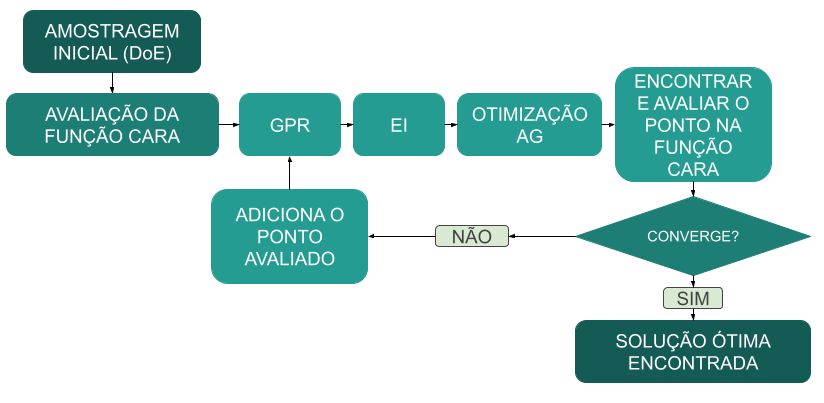
\includegraphics[width=0.7\linewidth]{figuras/fluxograma_EGO.png}
    \caption{Fluxograma operacional do EGO.}
    \label{fig:Fluxograma_EGO}
\end{figure}

Em forma objetiva, tem-se:
\begin{enumerate}
    \item \textbf{Projeto de Experimentos (DoE -- \textit{Design of Experiments}) inicial:} escolher um conjunto inicial $X$ com boa cobertura do domínio (por exemplo, \textit{Latin Hypercube}) e avaliar $Y$ \cite{Jones1998}.
    \item \textbf{Treinamento do \textit{surrogate}:} ajustar o modelo probabilístico aos dados $(X,Y)$ para obter $\mu(\mathbf{x})$ e $\sigma(\mathbf{x})$ (ou $\sigma^2(\mathbf{x})$) \cite{Jones1998}.
    \item \textbf{Construção da aquisição:} calcular $\mathrm{EI}(\mathbf{x})$.
    \item \textbf{Escolha do próximo ponto:} resolver
    \begin{equation}
        \mathbf{x}_{n+1}=\arg\max_{\mathbf{x}\in\mathcal{X}} \mathrm{EI}(\mathbf{x}),
    \end{equation}

    em que o termo $\arg\max$ retorna o ponto que maximiza a função. Em seguida avalia $y_{n+1}=F(\mathbf{x}_{n+1})$
    \item \textbf{Atualização:} incorporar $(\mathbf{x}_{n+1},y_{n+1})$ ao conjunto e repetir a partir do passo 2 \cite{Jones1998}.
\end{enumerate}

A iteração prossegue até um orçamento máximo de avaliações ou até que o ganho esperado se torne marginal (por exemplo, $\max_{\mathbf{x}}\mathrm{EI}(\mathbf{x})$ suficientemente pequeno), indicando baixo retorno incremental para novas amostras \cite{Jones1998,Shahriari2016}.





